% Practice Test 09 — Indiana Edition
% Questions: 30 (21 MC + 9 SA)
% Generated by scripts/generate_practice_tests.py

\begin{practiceQuestion}{1-3-q14}{mc}
\begin{questionText}
A recipe uses cups of flour proportional to servings. If $12$ servings need $9$ cups, what is $k$ in cups per serving?
\end{questionText}
\choiceA{$\frac{3}{4}$}
\choiceB{$\frac{4}{3}$}
\choiceC{$3$}
\choiceD{$9$}
\correctAnswer{A}
\explanation{$k = \frac{9}{12} = \frac{3}{4}$ cups per serving.}
\end{practiceQuestion}

\begin{practiceQuestion}{1-5-q10}{mc}
\begin{questionText}
A graph shows that $4$ gallons of paint covers $600$ square feet. The relationship is proportional. How many square feet does $1$ gallon cover?
\end{questionText}
\choiceA{$120$ sq ft}
\choiceB{$150$ sq ft}
\choiceC{$200$ sq ft}
\choiceD{$600$ sq ft}
\correctAnswer{B}
\explanation{Unit rate $= \frac{600}{4} = 150$ sq ft per gallon. This is the $y$-value at $x = 1$ on the graph.}
\end{practiceQuestion}

\begin{practiceQuestion}{1-6-q23}{sa}
\begin{questionText}
A garden hose fills a $60$-gallon tank in $8$ minutes. How long does it take to fill a $225$-gallon tank?
\end{questionText}
\correctAnswer{$30$ minutes}
\explanation{Rate: $60 \div 8 = 7.5$ gal/min. Time: $225 \div 7.5 = 30$ minutes.}
\end{practiceQuestion}

\begin{practiceQuestion}{2-2-q02}{mc}
\begin{questionText}
Use a proportion to find $35\%$ of $120$.
\end{questionText}
\choiceA{$35$}
\choiceB{$38$}
\choiceC{$42$}
\choiceD{$48$}
\correctAnswer{C}
\explanation{Set up $\frac{n}{120} = \frac{35}{100}$. Cross-multiply: $100n = 4200$. Divide: $n = 42$.}
\end{practiceQuestion}

\begin{practiceQuestion}{2-5-q15}{mc}
\begin{questionText}
An art dealer charges $12\%$ commission on each painting sold. If she sold a painting for $\$1{,}500$, what is the revenue for the artist (after the commission is taken)?
\end{questionText}
\choiceA{$\$180$}
\choiceB{$\$1{,}200$}
\choiceC{$\$1{,}320$}
\choiceD{$\$1{,}380$}
\correctAnswer{C}
\explanation{Commission: $1{,}500 \times 0.12 = \$180$. Artist gets: $1{,}500 - 180 = \$1{,}320$.}
\end{practiceQuestion}

\begin{practiceQuestion}{2-7-q06}{mc}
\begin{questionText}
Which estimate has a lower percent error?
\begin{itemize}
    \item Estimate A: guessed $45$, actual was $50$
    \item Estimate B: guessed $95$, actual was $100$
\end{itemize}
\end{questionText}
\choiceA{Estimate A ($10\%$ error)}
\choiceB{Estimate B ($5\%$ error)}
\choiceC{They have the same percent error}
\choiceD{Cannot be determined}
\correctAnswer{B}
\explanation{A: $\frac{5}{50} \times 100 = 10\%$. B: $\frac{5}{100} \times 100 = 5\%$. Estimate B has lower percent error.}
\end{practiceQuestion}

\begin{practiceQuestion}{3-1-q21}{sa}
\begin{questionText}
Order from least to greatest: $-7, \; 3, \; -1, \; 0, \; -4$.
\end{questionText}
\correctAnswer{$-7, \; -4, \; -1, \; 0, \; 3$}
\explanation{On a number line from left to right: $-7 < -4 < -1 < 0 < 3$.}
\end{practiceQuestion}

\begin{practiceQuestion}{3-2-q07}{mc}
\begin{questionText}
What is $(-3) + (-9) + 4$?
\end{questionText}
\choiceA{$-8$}
\choiceB{$-16$}
\choiceC{$10$}
\choiceD{$2$}
\correctAnswer{A}
\explanation{Add the negatives first: $(-3) + (-9) = -12$. Then $(-12) + 4 = -8$.}
\end{practiceQuestion}

\begin{practiceQuestion}{4-2-q19}{sa}
\begin{questionText}
Simplify $8p - 3 + 2p - 7$.
\end{questionText}
\correctAnswer{$10p - 10$}
\explanation{Combine variable terms: $8p + 2p = 10p$. Combine constants: $-3 - 7 = -10$. Result: $10p - 10$.}
\end{practiceQuestion}

\begin{practiceQuestion}{4-3-q28}{gmc}
\begin{questionText}
Three friends each receive the same gift bag containing $x$ stickers and $4$ erasers. The diagram below represents the total items.

\begin{center}
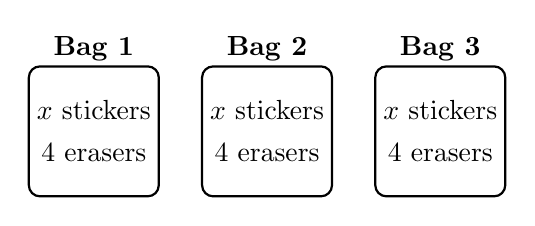
\begin{tikzpicture}[scale=0.55]
  % Bag 1
  \draw[thick, rounded corners] (0,0) rectangle (3,3);
  \node[font=\bfseries] at (1.5,3.4) {Bag 1};
  \node at (1.5,2) {$x$ stickers};
  \node at (1.5,1) {$4$ erasers};
  % Bag 2
  \draw[thick, rounded corners] (4,0) rectangle (7,3);
  \node[font=\bfseries] at (5.5,3.4) {Bag 2};
  \node at (5.5,2) {$x$ stickers};
  \node at (5.5,1) {$4$ erasers};
  % Bag 3
  \draw[thick, rounded corners] (8,0) rectangle (11,3);
  \node[font=\bfseries] at (9.5,3.4) {Bag 3};
  \node at (9.5,2) {$x$ stickers};
  \node at (9.5,1) {$4$ erasers};
\end{tikzpicture}
\end{center}

Which expression represents the total number of items?
\end{questionText}
\choiceA{$3x + 4$}
\choiceB{$x + 12$}
\choiceC{$3(x + 4) = 3x + 12$}
\choiceD{$3x + 4 + 4 + 4 = 3x + 4$}
\correctAnswer{C}
\explanation{Each bag has $x + 4$ items. With $3$ bags: $3(x + 4) = 3x + 12$ total items.}
\end{practiceQuestion}

\begin{practiceQuestion}{5-4-q26}{gmc}
\begin{questionText}
The table shows input and output values for a function. What is the rule?

\begin{center}
\begin{tabular}{|c|c|}
\hline
\textbf{Input ($x$)} & \textbf{Output ($y$)} \\
\hline
$2$ & $2.5$ \\
\hline
$4$ & $3.5$ \\
\hline
$6$ & $4.5$ \\
\hline
$10$ & $6.5$ \\
\hline
\end{tabular}
\end{center}
\end{questionText}
\choiceA{$y = 0.5x + 1.5$}
\choiceB{$y = x - 0.5$}
\choiceC{$y = 0.25x + 2$}
\choiceD{$y = 2x - 1.5$}
\correctAnswer{A}
\explanation{From $x = 2$ to $x = 4$, $y$ increases by $1$ while $x$ increases by $2$, so rate $= 0.5$. When $x = 2$: $0.5(2) + 1.5 = 2.5$ \checkmark.}
\end{practiceQuestion}

\begin{practiceQuestion}{5-5-q03}{mc}
\begin{questionText}
Which inequality represents ``at most $15$''?
\end{questionText}
\choiceA{$x > 15$}
\choiceB{$x < 15$}
\choiceC{$x \geq 15$}
\choiceD{$x \leq 15$}
\correctAnswer{D}
\explanation{``At most'' means $15$ or less, which is $x \leq 15$.}
\end{practiceQuestion}

\begin{practiceQuestion}{5-6-q10}{mc}
\begin{questionText}
Solve $5 - x > 8$ and describe the graph.
\end{questionText}
\choiceA{Open circle at $3$, shade right}
\choiceB{Open circle at $-3$, shade left}
\choiceC{Closed circle at $-3$, shade left}
\choiceD{Open circle at $-3$, shade right}
\correctAnswer{B}
\explanation{Subtract $5$: $-x > 3$. Multiply by $-1$ and flip: $x < -3$. Open circle at $-3$, shade left.}
\end{practiceQuestion}

\begin{practiceQuestion}{6-1-q28}{gmc}
\begin{questionText}
The scale drawing below shows a rectangular garden with scale $1$ cm $= 3$ m. Which statement is correct about the actual garden?

\begin{center}
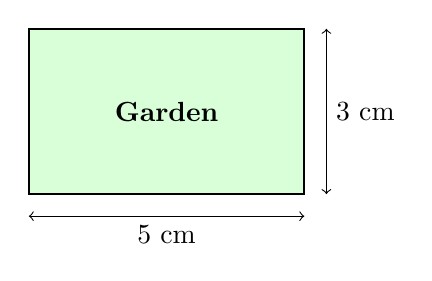
\begin{tikzpicture}[scale=0.7]
  \draw[thick,fill=green!15] (0,0) rectangle (5,3);
  \draw[<->] (0,-0.4) -- (5,-0.4);
  \node[below] at (2.5,-0.4) {$5$ cm};
  \draw[<->] (5.4,0) -- (5.4,3);
  \node[right] at (5.4,1.5) {$3$ cm};
  \node at (2.5,1.5) {\textbf{Garden}};
\end{tikzpicture}
\end{center}
\end{questionText}
\choiceA{The actual garden has an area of $15$ m$^2$}
\choiceB{The actual garden has a perimeter of $48$ m}
\choiceC{The actual garden has an area of $135$ m$^2$}
\choiceD{The actual garden has a perimeter of $16$ m}
\correctAnswer{C}
\explanation{Actual dimensions: $5 \times 3 = 15$ m and $3 \times 3 = 9$ m. Area: $15 \times 9 = 135$ m$^2$. Perimeter: $2(15 + 9) = 48$ m. Both B and C look plausible, but the area of $135$ m$^2$ matches choice C.}
\end{practiceQuestion}

\begin{practiceQuestion}{6-3-q03}{mc}
\begin{questionText}
A quadrilateral has four given side lengths: $3$, $4$, $5$, and $6$. How many different quadrilaterals can be drawn?
\end{questionText}
\choiceA{Exactly one}
\choiceB{Exactly two}
\choiceC{More than one}
\choiceD{None — it is impossible}
\correctAnswer{C}
\explanation{Four side lengths alone do not fix the angles of a quadrilateral. Many different shapes are possible with the same four sides.}
\end{practiceQuestion}

\begin{practiceQuestion}{6-4-q05}{mc}
\begin{questionText}
Which condition does NOT produce a unique triangle?
\end{questionText}
\choiceA{SSS with valid side lengths}
\choiceB{SAS}
\choiceC{ASA}
\choiceD{AAA}
\correctAnswer{D}
\explanation{AAA (three angles) determines the shape but allows infinitely many different sizes. SSS, SAS, and ASA each produce exactly one unique triangle.}
\end{practiceQuestion}

\begin{practiceQuestion}{6-5-q02}{mc}
\begin{questionText}
You slice a cylinder with a horizontal cut parallel to its base. What shape is the cross-section?
\end{questionText}
\choiceA{Rectangle}
\choiceB{Circle}
\choiceC{Oval}
\choiceD{Triangle}
\correctAnswer{B}
\explanation{A horizontal cut through a cylinder parallel to the circular base produces a circle.}
\end{practiceQuestion}

\begin{practiceQuestion}{6-6-q22}{sa}
\begin{questionText}
Two supplementary angles are in the ratio $5:4$. Find both angles.
\end{questionText}
\correctAnswer{$100°$ and $80°$}
\explanation{$5x + 4x = 180$. Combine: $9x = 180$. Solve: $x = 20$. Angles: $5(20) = 100°$ and $4(20) = 80°$.}
\end{practiceQuestion}

\begin{practiceQuestion}{6-7-q29}{gsa}
\begin{questionText}
The coordinate plane shows a rectangle with vertices $A(1, 1)$, $B(5, 1)$, $C(5, 3)$, $D(1, 3)$. Reflect the rectangle over the $x$-axis and list the new vertices.

\begin{center}
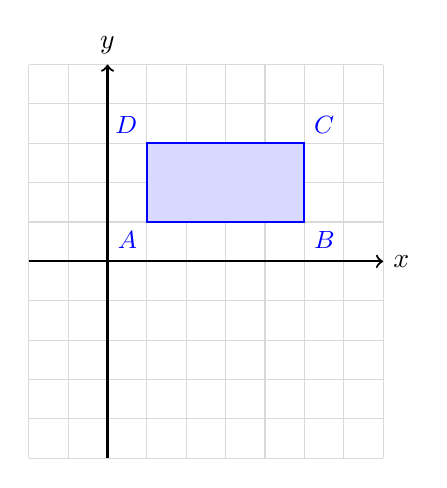
\begin{tikzpicture}[scale=0.5]
  \draw[step=1,gray!30,thin] (-2,-5) grid (7,5);
  \draw[thick,->] (-2,0) -- (7,0) node[right]{$x$};
  \draw[thick,->] (0,-5) -- (0,5) node[above]{$y$};
  \draw[thick,blue,fill=blue!15] (1,1) -- (5,1) -- (5,3) -- (1,3) -- cycle;
  \node[above left,blue,font=\small] at (1,3) {$D$};
  \node[above right,blue,font=\small] at (5,3) {$C$};
  \node[below left,blue,font=\small] at (1,1) {$A$};
  \node[below right,blue,font=\small] at (5,1) {$B$};
\end{tikzpicture}
\end{center}
\end{questionText}
\correctAnswer{$A'(1, -1)$, $B'(5, -1)$, $C'(5, -3)$, $D'(1, -3)$}
\explanation{Over the $x$-axis: keep $x$, negate $y$. $(1,1) \to (1,-1)$, $(5,1) \to (5,-1)$, $(5,3) \to (5,-3)$, $(1,3) \to (1,-3)$.}
\end{practiceQuestion}

\begin{practiceQuestion}{7-3-q12}{mc}
\begin{questionText}
Which circle has the larger area: Circle A with radius $4$ cm or Circle B with diameter $10$ cm?
\end{questionText}
\choiceA{Circle A}
\choiceB{Circle B}
\choiceC{They have the same area}
\choiceD{Not enough information}
\correctAnswer{B}
\explanation{Circle A: $r = 4$, $A = \pi(16) = 50.24$ cm$^2$. Circle B: $r = 5$, $A = \pi(25) = 78.5$ cm$^2$. Circle B is larger.}
\end{practiceQuestion}

\begin{practiceQuestion}{7-4-q03}{mc}
\begin{questionText}
A shape is made of two rectangles. Rectangle A is $6$ m by $3$ m and Rectangle B is $4$ m by $3$ m. What is the total area?
\end{questionText}
\choiceA{$18$ m$^2$}
\choiceB{$24$ m$^2$}
\choiceC{$30$ m$^2$}
\choiceD{$72$ m$^2$}
\correctAnswer{C}
\explanation{Rectangle A: $6 \times 3 = 18$ m$^2$. Rectangle B: $4 \times 3 = 12$ m$^2$. Total: $18 + 12 = 30$ m$^2$.}
\end{practiceQuestion}

\begin{practiceQuestion}{7-5-q23}{sa}
\begin{questionText}
A shipping box is $12$ in by $8$ in by $6$ in. What is the total surface area?
\end{questionText}
\correctAnswer{$432$ in$^2$}
\explanation{$SA = 2(12 \times 8) + 2(12 \times 6) + 2(8 \times 6) = 192 + 144 + 96 = 432$ in$^2$.}
\end{practiceQuestion}

\begin{practiceQuestion}{7-6-q24}{sa}
\begin{questionText}
A planter box is $3$ ft long, $1.5$ ft wide, and $2$ ft deep. How many cubic feet of soil are needed to fill it?
\end{questionText}
\correctAnswer{$9$ ft$^3$}
\explanation{$V = 3 \times 1.5 \times 2 = 9$ ft$^3$.}
\end{practiceQuestion}

\begin{practiceQuestion}{8-1-q19}{sa}
\begin{questionText}
A random sample of $80$ out of $2{,}000$ students found that $20$ students ride the bus. Predict how many students in the school ride the bus.
\end{questionText}
\correctAnswer{$500$}
\explanation{$\frac{20}{80} = 25\%$. Then $25\%$ of $2{,}000 = 500$.}
\end{practiceQuestion}

\begin{practiceQuestion}{8-3-q04}{mc}
\begin{questionText}
Group X has a median of $50$ and a range of $10$. Group Y has a median of $50$ and a range of $30$. Which statement is true?
\end{questionText}
\choiceA{Group X has more data values}
\choiceB{Group Y has a higher center}
\choiceC{Group Y is more spread out than Group X}
\choiceD{The groups are identical}
\correctAnswer{C}
\explanation{Both have the same median, but Group Y's larger range means its data is more spread out.}
\end{practiceQuestion}

\begin{practiceQuestion}{8-4-q01}{mc}
\begin{questionText}
Data set A: $10, 12, 14, 16, 18$. What is the mean?
\end{questionText}
\choiceA{$12$}
\choiceB{$14$}
\choiceC{$16$}
\choiceD{$70$}
\correctAnswer{B}
\explanation{$\frac{10+12+14+16+18}{5} = \frac{70}{5} = 14$.}
\end{practiceQuestion}

\begin{practiceQuestion}{8-7-q07}{mc}
\begin{questionText}
In a double bar graph, Team X scored $30$, $45$, $50$ over three games and Team Y scored $35$, $40$, $55$. What was Team Y's total?
\end{questionText}
\choiceA{$120$}
\choiceB{$125$}
\choiceC{$130$}
\choiceD{$135$}
\correctAnswer{C}
\explanation{$35 + 40 + 55 = 130$.}
\end{practiceQuestion}

\begin{practiceQuestion}{9-4-q25}{sa}
\begin{questionText}
A probability model assigns $P(A) = 0.35$, $P(B) = 0.25$, $P(C) = 0.25$, and $P(D) = 0.20$. Is this a valid model? Explain.
\end{questionText}
\correctAnswer{No}
\explanation{$0.35 + 0.25 + 0.25 + 0.20 = 1.05$, which is greater than $1$. A valid model must have probabilities that sum to exactly $1$.}
\end{practiceQuestion}

\begin{practiceQuestion}{9-6-q14}{mc}
\begin{questionText}
A bag has $4$ green and $6$ yellow marbles. You pick one marble without replacement and then pick another. What is the probability that the first is green and the second is yellow?
\end{questionText}
\choiceA{$\frac{24}{100}$}
\choiceB{$\frac{24}{90}$}
\choiceC{$\frac{4}{15}$}
\choiceD{$\frac{6}{10}$}
\correctAnswer{C}
\explanation{$P(\text{green first}) = \frac{4}{10}$. After removing a green, $P(\text{yellow second}) = \frac{6}{9}$. $P = \frac{4}{10} \times \frac{6}{9} = \frac{24}{90} = \frac{4}{15}$.}
\end{practiceQuestion}

\begin{practiceQuestion}{9-7-q06}{mc}
\begin{questionText}
Why are simulations useful?
\end{questionText}
\choiceA{They always give exact answers}
\choiceB{They can estimate probabilities when real experiments are too difficult or impractical}
\choiceC{They replace all mathematical calculations}
\choiceD{They only work for coin flips}
\correctAnswer{B}
\explanation{Simulations estimate probabilities for complex events that are hard to compute directly or where real experiments are impractical.}
\end{practiceQuestion}
